\documentclass[11pt]{article}
\usepackage{arxiv}
\usepackage{amsfonts}
\usepackage{amsmath}
\usepackage{amsthm}
\usepackage{pxfonts}
\usepackage{mathtools}
\usepackage{tocloft}
\usepackage{dsfont}
\usepackage{todonotes}%loads xcolor with []
\usepackage{extarrows}
\usepackage{titlesec}
\usepackage{enumitem}

\usepackage{wrapfig}
\usepackage{caption}


\usepackage{hyperref}
\usepackage{subcaption}

% Definitions of handy macros can go here
\newcommand{\toodoo}[1]{{\tt\color{red} #1}}

\theoremstyle{definition}
\newtheorem{definition}{Definition}[]
\newtheorem{example}[definition]{Example}
\newtheorem{remark}[definition]{Remark}
\newtheorem{setting}[definition]{Setting}
\newtheorem{assumption}[definition]{Assumption}
\newtheorem{hypothesis}[definition]{Hypothesis}
\theoremstyle{plain}
\newtheorem{theorem}[definition]{Theorem}
\newtheorem{corollary}[definition]{Corollary}
\newtheorem{proposition}[definition]{Proposition}
\newtheorem{lemma}[definition]{Lemma}

\renewcommand{\labelenumi}{\textup{(\textit{\roman{enumi}})}}
\setlength\cftparskip{0pt}
\setlength\cftbeforesecskip{2pt}

\newcommand{\N}{\mathbb{N}}
\newcommand{\bm}[1]{\boldsymbol{#1}}
\newcommand{\Rn}{\R^n}
\newcommand{\dx}{\mathrm{d}x}
\newcommand{\rami}[1]{\textcolor{blue}{#1}}

\newcommand{\norm}[1]{\left\lVert#1\right\rVert}

% requirements
\usepackage{amsmath}
\usepackage{amssymb}
\usepackage{bm}
\usepackage{mathtools}

% Random variables
\def\reta{{\textnormal{$\eta$}}}
\def\ra{{\textnormal{a}}}
\def\rb{{\textnormal{b}}}
\def\rc{{\textnormal{c}}}
\def\rd{{\textnormal{d}}}
\def\re{{\textnormal{e}}}
\def\rf{{\textnormal{f}}}
\def\rg{{\textnormal{g}}}
\def\rh{{\textnormal{h}}}
\def\ri{{\textnormal{i}}}
\def\rj{{\textnormal{j}}}
\def\rk{{\textnormal{k}}}
\def\rl{{\textnormal{l}}}
% rm is already a command, just don't name any random variables m
\def\rn{{\textnormal{n}}}
\def\ro{{\textnormal{o}}}
\def\rp{{\textnormal{p}}}
\def\rq{{\textnormal{q}}}
\def\rr{{\textnormal{r}}}
\def\rs{{\textnormal{s}}}
\def\rt{{\textnormal{t}}}
\def\ru{{\textnormal{u}}}
\def\rv{{\textnormal{v}}}
\def\rw{{\textnormal{w}}}
\def\rx{{\textnormal{x}}}
\def\ry{{\textnormal{y}}}
\def\rz{{\textnormal{z}}}

% Random vectors
\def\rvepsilon{{\mathbf{\epsilon}}}
\def\rvtheta{{\mathbf{\theta}}}
\def\rva{{\mathbf{a}}}
\def\rvb{{\mathbf{b}}}
\def\rvc{{\mathbf{c}}}
\def\rvd{{\mathbf{d}}}
\def\rve{{\mathbf{e}}}
\def\rvf{{\mathbf{f}}}
\def\rvg{{\mathbf{g}}}
\def\rvh{{\mathbf{h}}}
\def\rvu{{\mathbf{i}}}
\def\rvj{{\mathbf{j}}}
\def\rvk{{\mathbf{k}}}
\def\rvl{{\mathbf{l}}}
\def\rvm{{\mathbf{m}}}
\def\rvn{{\mathbf{n}}}
\def\rvo{{\mathbf{o}}}
\def\rvp{{\mathbf{p}}}
\def\rvq{{\mathbf{q}}}
\def\rvr{{\mathbf{r}}}
\def\rvs{{\mathbf{s}}}
\def\rvt{{\mathbf{t}}}
\def\rvu{{\mathbf{u}}}
\def\rvv{{\mathbf{v}}}
\def\rvw{{\mathbf{w}}}
\def\rvx{{\mathbf{x}}}
\def\rvy{{\mathbf{y}}}
\def\rvz{{\mathbf{z}}}

% Elements of random vectors
\def\erva{{\textnormal{a}}}
\def\ervb{{\textnormal{b}}}
\def\ervc{{\textnormal{c}}}
\def\ervd{{\textnormal{d}}}
\def\erve{{\textnormal{e}}}
\def\ervf{{\textnormal{f}}}
\def\ervg{{\textnormal{g}}}
\def\ervh{{\textnormal{h}}}
\def\ervi{{\textnormal{i}}}
\def\ervj{{\textnormal{j}}}
\def\ervk{{\textnormal{k}}}
\def\ervl{{\textnormal{l}}}
\def\ervm{{\textnormal{m}}}
\def\ervn{{\textnormal{n}}}
\def\ervo{{\textnormal{o}}}
\def\ervp{{\textnormal{p}}}
\def\ervq{{\textnormal{q}}}
\def\ervr{{\textnormal{r}}}
\def\ervs{{\textnormal{s}}}
\def\ervt{{\textnormal{t}}}
\def\ervu{{\textnormal{u}}}
\def\ervv{{\textnormal{v}}}
\def\ervw{{\textnormal{w}}}
\def\ervx{{\textnormal{x}}}
\def\ervy{{\textnormal{y}}}
\def\ervz{{\textnormal{z}}}

% Random matrices
\def\rmA{{\mathbf{A}}}
\def\rmB{{\mathbf{B}}}
\def\rmC{{\mathbf{C}}}
\def\rmD{{\mathbf{D}}}
\def\rmE{{\mathbf{E}}}
\def\rmF{{\mathbf{F}}}
\def\rmG{{\mathbf{G}}}
\def\rmH{{\mathbf{H}}}
\def\rmI{{\mathbf{I}}}
\def\rmJ{{\mathbf{J}}}
\def\rmK{{\mathbf{K}}}
\def\rmL{{\mathbf{L}}}
\def\rmM{{\mathbf{M}}}
\def\rmN{{\mathbf{N}}}
\def\rmO{{\mathbf{O}}}
\def\rmP{{\mathbf{P}}}
\def\rmQ{{\mathbf{Q}}}
\def\rmR{{\mathbf{R}}}
\def\rmS{{\mathbf{S}}}
\def\rmT{{\mathbf{T}}}
\def\rmU{{\mathbf{U}}}
\def\rmV{{\mathbf{V}}}
\def\rmW{{\mathbf{W}}}
\def\rmX{{\mathbf{X}}}
\def\rmY{{\mathbf{Y}}}
\def\rmZ{{\mathbf{Z}}}

% Elements of random matrices
\def\ermA{{\textnormal{A}}}
\def\ermB{{\textnormal{B}}}
\def\ermC{{\textnormal{C}}}
\def\ermD{{\textnormal{D}}}
\def\ermE{{\textnormal{E}}}
\def\ermF{{\textnormal{F}}}
\def\ermG{{\textnormal{G}}}
\def\ermH{{\textnormal{H}}}
\def\ermI{{\textnormal{I}}}
\def\ermJ{{\textnormal{J}}}
\def\ermK{{\textnormal{K}}}
\def\ermL{{\textnormal{L}}}
\def\ermM{{\textnormal{M}}}
\def\ermN{{\textnormal{N}}}
\def\ermO{{\textnormal{O}}}
\def\ermP{{\textnormal{P}}}
\def\ermQ{{\textnormal{Q}}}
\def\ermR{{\textnormal{R}}}
\def\ermS{{\textnormal{S}}}
\def\ermT{{\textnormal{T}}}
\def\ermU{{\textnormal{U}}}
\def\ermV{{\textnormal{V}}}
\def\ermW{{\textnormal{W}}}
\def\ermX{{\textnormal{X}}}
\def\ermY{{\textnormal{Y}}}
\def\ermZ{{\textnormal{Z}}}

% Vectors
\def\vzero{{\bm{0}}}
\def\vone{{\bm{1}}}
\def\vmu{{\bm{\mu}}}
\def\vnu{{\bm{\nu}}}
\def\vtheta{{\bm{\theta}}}
\def\vepsilon{{\bm{\epsilon}}}
\def\vgamma{{\bm{\gamma}}}
\def\vdelta{{\bm{\delta}}}
\def\vDelta{{\bm{\Delta}}}
\def\va{{\bm{a}}}
\def\vb{{\bm{b}}}
\def\vc{{\bm{c}}}
\def\vd{{\bm{d}}}
\def\ve{{\bm{e}}}
\def\vetilde{\bm{\tilde{e}}}
\def\vell{{\bm{\ell}}}
\def\vf{{\bm{f}}}
\def\vg{{\bm{g}}}
\def\vh{{\bm{h}}}
\def\vi{{\bm{i}}}
\def\vj{{\bm{j}}}
\def\vk{{\bm{k}}}
\def\vl{{\bm{l}}}
\def\vm{{\bm{m}}}
\def\vmhat{{\bm{\hat{m}}}}
\def\vn{{\bm{n}}}
\def\vo{{\bm{o}}}
\def\vp{{\bm{p}}}
\def\vphi{{\bm{\phi}}}
\def\vq{{\bm{q}}}
\def\vr{{\bm{r}}}
\def\vs{{\bm{s}}}
\def\vstilde{\bm{\tilde{s}}}
\def\vt{{\bm{t}}}
\def\vu{{\bm{u}}}
\def\vv{{\bm{v}}}
\def\vvhat{{\bm{\hat{v}}}}
\def\vw{{\bm{w}}}
\def\vx{{\bm{x}}}
\def\vy{{\bm{y}}}
\def\vytilde{{\bm{\tilde{y}}}}
\def\vyhat{{\bm{\hat{y}}}}
\def\vz{{\bm{z}}}

% Elements of vectors
\def\evalpha{{\alpha}}
\def\evbeta{{\beta}}
\def\evepsilon{{\epsilon}}
\def\evlambda{{\lambda}}
\def\evomega{{\omega}}
\def\evmu{{\mu}}
\def\evpsi{{\psi}}
\def\evsigma{{\sigma}}
\def\evtheta{{\theta}}
\def\eva{{a}}
\def\evb{{b}}
\def\evc{{c}}
\def\evd{{d}}
\def\eve{{e}}
\def\evf{{f}}
\def\evg{{g}}
\def\evh{{h}}
\def\evi{{i}}
\def\evj{{j}}
\def\evk{{k}}
\def\evl{{l}}
\def\evm{{m}}
\def\evn{{n}}
\def\evo{{o}}
\def\evp{{p}}
\def\evq{{q}}
\def\evr{{r}}
\def\evs{{s}}
\def\evt{{t}}
\def\evu{{u}}
\def\evv{{v}}
\def\evw{{w}}
\def\evx{{x}}
\def\evy{{y}}
\def\evyhat{{\hat{y}}}
\def\evz{{z}}

% Matrix
\def\mA{{\bm{A}}}
\def\mB{{\bm{B}}}
\def\mC{{\bm{C}}}
\def\mD{{\bm{D}}}
\def\mE{{\bm{E}}}
\def\mF{{\bm{F}}}
\def\mG{{\bm{G}}}
\def\mGtilde{\bm{\tilde{G}}}
\def\mH{{\bm{H}}}
\def\mI{{\bm{I}}}
\def\mJ{{\bm{J}}}
\def\mK{{\bm{K}}}
\def\mL{{\bm{L}}}
\def\mM{{\bm{M}}}
\def\mN{{\bm{N}}}
\def\mO{{\bm{O}}}
\def\mP{{\bm{P}}}
\def\mQ{{\bm{Q}}}
\def\mR{{\bm{R}}}
\def\mS{{\bm{S}}}
\def\mT{{\bm{T}}}
\def\mU{{\bm{U}}}
\def\mV{{\bm{V}}}
\def\mW{{\bm{W}}}
\def\mX{{\bm{X}}}
\def\mY{{\bm{Y}}}
\def\mZ{{\bm{Z}}}
\def\mBeta{{\bm{\beta}}}
\def\mGamma{{\bm{\Gamma}}}
\def\mPhi{{\bm{\Phi}}}
\def\mPi{{\bm{\Pi}}}
\def\mLambda{{\bm{\Lambda}}}
\def\mSigma{{\bm{\Sigma}}}
\def\mOmega{{\bm{\Omega}}}
\def\mStilde{\bm{\tilde{\mS}}}
\def\mGtilde{\bm{\tilde{\mG}}}
\def\mGoverline{{\bm{\overline{G}}}}

% Tensor
\DeclareMathAlphabet{\mathsfit}{\encodingdefault}{\sfdefault}{m}{sl}
\SetMathAlphabet{\mathsfit}{bold}{\encodingdefault}{\sfdefault}{bx}{n}
\newcommand{\tens}[1]{\bm{\mathsfit{#1}}}
\def\tA{{\tens{A}}}
\def\tB{{\tens{B}}}
\def\tC{{\tens{C}}}
\def\tD{{\tens{D}}}
\def\tE{{\tens{E}}}
\def\tF{{\tens{F}}}
\def\tG{{\tens{G}}}
\def\tH{{\tens{H}}}
\def\tI{{\tens{I}}}
\def\tJ{{\tens{J}}}
\def\tK{{\tens{K}}}
\def\tL{{\tens{L}}}
\def\tM{{\tens{M}}}
\def\tN{{\tens{N}}}
\def\tO{{\tens{O}}}
\def\tP{{\tens{P}}}
\def\tPi{\bm{\mathsf{\Pi}}}
\def\tQ{{\tens{Q}}}
\def\tR{{\tens{R}}}
\def\tS{{\tens{S}}}
\def\tT{{\tens{T}}}
\def\tU{{\tens{U}}}
\def\tV{{\tens{V}}}
\def\tW{{\tens{W}}}
\def\tX{{\tens{X}}}
\def\tY{{\tens{Y}}}
\def\tZ{{\tens{Z}}}

% Graph
\def\gA{{\mathcal{A}}}
\def\gB{{\mathcal{B}}}
\def\gC{{\mathcal{C}}}
\def\gD{{\mathcal{D}}}
\def\gE{{\mathcal{E}}}
\def\gF{{\mathcal{F}}}
\def\gG{{\mathcal{G}}}
\def\gH{{\mathcal{H}}}
\def\gI{{\mathcal{I}}}
\def\gJ{{\mathcal{J}}}
\def\gK{{\mathcal{K}}}
\def\gL{{\mathcal{L}}}
\def\gM{{\mathcal{M}}}
\def\gN{{\mathcal{N}}}
\def\gO{{\mathcal{O}}}
\def\gP{{\mathcal{P}}}
\def\gQ{{\mathcal{Q}}}
\def\gR{{\mathcal{R}}}
\def\gS{{\mathcal{S}}}
\def\gT{{\mathcal{T}}}
\def\gU{{\mathcal{U}}}
\def\gV{{\mathcal{V}}}
\def\gW{{\mathcal{W}}}
\def\gX{{\mathcal{X}}}
\def\gY{{\mathcal{Y}}}
\def\gZ{{\mathcal{Z}}}

% Sets
\def\sA{{\mathbb{A}}}
\def\sB{{\mathbb{B}}}
\def\sC{{\mathbb{C}}}
\def\sD{{\mathbb{D}}}
% Don't use a set called E, because this would be the same as our symbol
% for expectation.
\def\sF{{\mathbb{F}}}
\def\sG{{\mathbb{G}}}
\def\sH{{\mathbb{H}}}
\def\sI{{\mathbb{I}}}
\def\sJ{{\mathbb{J}}}
\def\sK{{\mathbb{K}}}
\def\sL{{\mathbb{L}}}
\def\sM{{\mathbb{M}}}
\def\sN{{\mathbb{N}}}
\def\sO{{\mathbb{O}}}
\def\sP{{\mathbb{P}}}
\def\sQ{{\mathbb{Q}}}
\def\sR{{\mathbb{R}}}
\def\sS{{\mathbb{S}}}
\def\sT{{\mathbb{T}}}
\def\sU{{\mathbb{U}}}
\def\sV{{\mathbb{V}}}
\def\sW{{\mathbb{W}}}
\def\sX{{\mathbb{X}}}
\def\sY{{\mathbb{Y}}}
\def\sYhat{{\hat{\mathbb{Y}}}}
\def\sZ{{\mathbb{Z}}}
% Blackboard Greek characters: https://tex.stackexchange.com/a/3260
\DeclareSymbolFont{bbold}{U}{bbold}{m}{n}
\DeclareSymbolFontAlphabet{\mathbbold}{bbold}
\def\sTheta{{\mathbbold{\Theta}}}
\def\sOmega{{\mathbbold{\Omega}}}

% Entries of a matrix
\def\emLambda{{\Lambda}}
\def\emA{{A}}
\def\emB{{B}}
\def\emC{{C}}
\def\emD{{D}}
\def\emE{{E}}
\def\emF{{F}}
\def\emG{{G}}
\def\emH{{H}}
\def\emI{{I}}
\def\emJ{{J}}
\def\emK{{K}}
\def\emL{{L}}
\def\emM{{M}}
\def\emN{{N}}
\def\emO{{O}}
\def\emP{{P}}
\def\emQ{{Q}}
\def\emR{{R}}
\def\emS{{S}}
\def\emT{{T}}
\def\emU{{U}}
\def\emV{{V}}
\def\emW{{W}}
\def\emX{{X}}
\def\emY{{Y}}
\def\emZ{{Z}}
\def\emSigma{{\Sigma}}
\def\emPi{{\Pi}}

% entries of a tensor
% Same font as tensor, without \bm wrapper
\newcommand{\etens}[1]{\mathsfit{#1}}
\def\etLambda{{\etens{\Lambda}}}
\def\etA{{\etens{A}}}
\def\etB{{\etens{B}}}
\def\etC{{\etens{C}}}
\def\etD{{\etens{D}}}
\def\etE{{\etens{E}}}
\def\etF{{\etens{F}}}
\def\etG{{\etens{G}}}
\def\etH{{\etens{H}}}
\def\etI{{\etens{I}}}
\def\etJ{{\etens{J}}}
\def\etK{{\etens{K}}}
\def\etL{{\etens{L}}}
\def\etM{{\etens{M}}}
\def\etN{{\etens{N}}}
\def\etO{{\etens{O}}}
\def\etP{{\etens{P}}}
\def\etPi{\mathsf{\Pi}}
\def\etQ{{\etens{Q}}}
\def\etR{{\etens{R}}}
\def\etS{{\etens{S}}}
\def\etT{{\etens{T}}}
\def\etU{{\etens{U}}}
\def\etV{{\etens{V}}}
\def\etW{{\etens{W}}}
\def\etX{{\etens{X}}}
\def\etY{{\etens{Y}}}
\def\etZ{{\etens{Z}}}

% The true underlying data generating distribution
\newcommand{\pdata}{p_{\mathrm{data}}}
% The empirical distribution defined by the training set
\newcommand{\ptrain}{\hat{p}_{\mathrm{data}}}
\newcommand{\Ptrain}{\hat{P}_{\mathrm{data}}}
% The model distribution
\newcommand{\pmodel}{p_{\rm{model}}}
\newcommand{\Pmodel}{P_{\rm{model}}}
\newcommand{\ptildemodel}{\tilde{p}_{\rm{model}}}
% Stochastic autoencoder distributions
\newcommand{\pencode}{p_{\rm{encoder}}}
\newcommand{\pdecode}{p_{\rm{decoder}}}
\newcommand{\precons}{p_{\rm{reconstruct}}}

\newcommand{\laplace}{\mathrm{Laplace}} % Laplace distribution

\newcommand{\E}{\mathbb{E}}
\newcommand{\Ls}{\mathcal{L}}
\newcommand{\R}{\mathbb{R}}
\newcommand{\emp}{\tilde{p}}
\newcommand{\lr}{\alpha}
\newcommand{\reg}{\lambda}
\newcommand{\rect}{\mathrm{rectifier}}
\newcommand{\softmax}{\mathrm{softmax}}
\newcommand{\onehot}{\mathrm{onehot}}
\newcommand{\sigmoid}{\sigma}
\newcommand{\softplus}{\zeta}
\newcommand{\KL}{D_{\mathrm{KL}}}
\newcommand{\Var}{\mathrm{Var}}
\newcommand{\standarderror}{\mathrm{SE}}
\newcommand{\Cov}{\mathrm{Cov}}
% Wolfram Mathworld says $L^2$ is for function spaces and $\ell^2$ is for vectors
% But then they seem to use $L^2$ for vectors throughout the site, and so does
% wikipedia.
\newcommand{\normlzero}{L^0}
\newcommand{\normlone}{L^1}
\newcommand{\normltwo}{L^2}
\newcommand{\normlp}{L^p}
\newcommand{\normmax}{L^\infty}

\newcommand{\parents}{Pa} % See usage in notation.tex. Chosen to match Daphne's book.

\DeclareMathOperator*{\argmax}{arg\,max}
\DeclareMathOperator*{\argmin}{arg\,min}
\DeclareMathOperator*{\minimize}{minimize}
\DeclareMathOperator*{\maximize}{maximize}

\DeclareMathOperator{\sign}{sign}
\DeclareMathOperator{\mean}{mean}
\DeclareMathOperator{\vmap}{vmap}
\DeclareMathOperator{\reshape}{reshape}
\DeclareMathOperator{\Tr}{Tr}
\DeclareMathOperator{\diag}{diag}
\DeclareMathOperator{\eig}{eig}
\DeclareMathOperator{\rank}{rank}
\DeclareMathOperator{\vecspan}{span}
\DeclareMathOperator{\overlap}{overlap}
\DeclareMathOperator{\Cat}{Cat}

%%%%% NEW MATH DEFINITIONS %%%%%
\newcommand{\jac}{\mathrm{J}}
\newcommand{\grad}[1]{\ensuremath{\nabla_{\!{#1}}}}
\newcommand{\gradsquared}[1]{\ensuremath{\nabla_{\!{#1}}^{2}}}

% || for KLDivergence
\DeclarePairedDelimiterX{\KLdivx}[2]{(}{)}{%
  #1\;\delimsize\|\;#2%
}
\newcommand{\KLdiv}{\KL\KLdivx}

% | for a | b
\newcommand{\giventhat}[2]{#1\;|\;#2}

\let\ab\allowbreak
%%% Local Variables:
%%% mode: latex
%%% TeX-master: "../main"
%%% End:
 % follow DL notation from the Goodfellow book
% ===================================================================
% MATH
% ===================================================================
\usepackage{nicefrac} % fractions that fit into inline text

% ===================================================================
% REFERENCES
% ===================================================================
\usepackage{cleveref} % automatically adds type of reference, MUST BE LOADED AFTER AMSMATH

%%% Local Variables:
%%% mode: latex
%%% TeX-master: "../main"
%%% End:


\title{Kfac PINNs }
\date{November 2022}

\author{Felix Dangel, Johannes M\"uller \& Marius Zeinhofer}

\begin{document}

\maketitle

\begin{abstract}
  Kfac for PINNs.
\end{abstract}
\section{Introduction}
PINNs are difficult to optimize.

\section{The Gramian/Fischer for the PINN Formulation of the Poisson Equation}
$\bullet$ I think most of the complexity can already be understood just from this example.
I illustrate, using the Poisson equation how to write the Gramian/Fisher as the product of a Jacobian and its transpose, see equation \eqref{eq:Jacobian_Fischer}.
Is this what you were after Felix?
I think it differs from the standard setting in the sense that suddenly the Laplacian shows up.
It can also be used to derive a matrix-free version of the energy natural gradient descent, like done in Hessian free optimization.
$\bullet$ We consider the Poisson equation
\begin{align*}
  -\Delta u & = f \quad \text{in }\Omega \\
  u & = g \quad \text{on }\partial\Omega
\end{align*}
where $f\in L^2(\Omega)$ and $g\in H^{3/2}(\partial\Omega)$ are some given rhs and boundary values.

$\bullet$ The function space energy is given by
\[ E(u) = \frac{1}{2} \int_\Omega (\Delta u + f) \mathrm dx + \frac12 \int_{\partial\Omega} (u-g)^2 \mathrm ds. \]

$\bullet$ The PINN loss, with discretized integrals, is
\begin{align*}
  L(\theta)
  &=
    \frac{1}{2N_\Omega} L_\Omega(\theta) + \frac{1}{2N_{\partial\Omega}}L_{\partial\Omega}(\theta)
  \\
  &=
    \frac{1}{2N_\Omega} \sum_{i=1}^{N_\Omega} (\Delta u_\theta(x_i) + f(x_i))^2 + \frac{1}{2N_{\partial\Omega}}\sum_{i=1}^{N_{\partial\Omega}} ( u_\theta(x^b_i) - g(x^b_i))^2
\end{align*}
where we denote by $(x_i)$, $i=1,\dots,N_\Omega$ the points in the interior of $\Omega$ and by $(x^b_i)$, $i=1,\dots,N_{\partial\Omega}$ the points on the boundary.
We need quite a lot of these points in practice, it can be in the thousands.
And we need them in one batch, too.

$\bullet$ The energy natural gradient is for this example to use the Fischer/Gramian of the form
\begin{equation*}
  F(\theta) = F_\Omega(\theta) + F_{\partial\Omega}(\theta)
\end{equation*}
where
\begin{equation}
  F_\Omega(\theta)_{ij} = \frac1{{N_\Omega}} \sum_{k=1}^{N_\Omega} \partial_{\theta_i} \Delta u_\theta(x_k) \partial_{\theta_j} \Delta u_\theta(x_k)
  % = \frac1{{N_\Omega}} \sum_{i=1}^{N_\Omega} (\partial_{\theta_i} f_\theta) (\partial_{\theta_j} f_\theta ),
\end{equation}
% where $f_\theta = \Delta u_\theta$.
and
\begin{equation}
  F_{\partial\Omega}(\theta)_{ij} = \frac1{{N_\Omega}} \sum_{k=1}^{N_{\partial\Omega}} \partial_{\theta_i} \Delta u_\theta(x_k^b) \partial_{\theta_j} \Delta u_\theta (x_k^b).
  % = \frac1{{N_\Omega}} \sum_{i=1}^{N_\Omega} (\partial_{\theta_i} f_\theta) (\partial_{\theta_j} f_\theta ),
\end{equation}
In more compact form and written as Jacobian products, this can be expressed as
\begin{equation}\label{eq:Jacobian_Fischer}
  F_\Omega(\theta) = Dr_\Omega(\theta)^T \cdot Dr_\Omega(\theta)
  \quad \text{and} \quad
  F_{\partial\Omega}(\theta) = Dr_{\partial\Omega}(\theta)^T \cdot Dr_{\partial\Omega}(\theta).
\end{equation}
Here, $Dr_\Omega(\theta)$ and $Dr_{\partial\Omega}(\theta)$  denote the \emph{Jacobians} of the maps
\begin{equation*}
  r_{\Omega}: \Theta \to \mathbb{R}^{N_\Omega}, \quad r_{\Omega}(\theta) = \frac{1}{\sqrt{N_{\Omega}}}(\Delta u_\theta(x_1), \dots, \Delta u_\theta(x_{N_{\Omega}}))
\end{equation*}
and
\begin{equation*}
  r_{\partial\Omega}: \Theta \to \mathbb{R}^{N_\partial\Omega}, \quad r_{\partial\Omega}(\theta) = \frac{1}{\sqrt{N_{\partial\Omega}}}(u_\theta(x^b_1), \dots, u_\theta(x^b_{N_{\partial\Omega}}))
\end{equation*}

\section{K-FAC for a shallow network}
Consider a shallow network
\[ u_\theta(x) = W_2\sigma(W_1 x), \]
where $x\in\mathbb R^d$, $W_1\in\mathbb R^{m\times d}, W_2\in\mathbb R^{1\times m}$.

\paragraph{Task: }
Understand the structure, in particular the computational graph of $f_\theta = \Delta u_\theta$.

\paragraph{One dimensional case: }
Assume first that $d=1$.
Then
\[ D_x u_\theta(x) = W_2 \operatorname{diag}(\sigma'(W_1 x)) W_1 \]
and
\[ D^2_x u_\theta(x) = W_2%(W_1^\top\otimes W_2)
  \operatorname{diag}(\operatorname{diag}(\sigma''(W_1 x)) W_1)W_1. % = W_2 \operatorname{diag}\sigma''(W_1 x) W_1^2 = W_2\odot W_1^2 \sigma''(W_1x),
\]
In another form
\[D^2 u_\theta(x) = W_2 \operatorname{diag}(\operatorname{diag}\sigma''(W_1 x) W_1) W_1 = W_2 \operatorname{diag}\sigma''(W_1 x) W_1^2 = W_2\odot W_1^2 \sigma''(W_1x),
\]
where $(W_2\odot W_1^2)_k = (W_2)_k \cdot (W_1)_k^2$.
% where $(W_2\odot W_1^2)_k = (W_2)_k \cdot (W_1)_k^2$.
% The Laplacian is then given as
% \[ f_\theta(x) = \Delta u_\theta(x) = \operatorname{tr}(D_x^2u_\theta(x)) =\operatorname{tr}(W_2 \operatorname{diag}(\operatorname{diag}(\sigma''(W_1 x)) W_1) W_1).  \]
% Differentiation with respect to $W_2$ yields
% \[ \frac{\partial f_\theta(x)}{\partial W_2} = \frac{\partial \Delta u_\theta(x)}{ \partial W_2} =  \]

One can also rewrite the diagonalization operator via a Hadamard product as $\operatorname{diag}(x) = (x\mathds{1}^\top)\odot I$, where $\mathds{1}$ denotes the all one vector, $I$ the identity and $\odot$ the Hadamard (i.e., entrywise) product of two matrices.
Not sure whether this helps though...

% \paragraph{One dimensional case: }

\section{Generalization to other PDEs}
Essential to the formula above is that the discrete bilinear form (not explicitly stated above) can be written in the way
\begin{equation}\label{eq:gramian_asssumption}
  a^h(u,v)
  =
  \langle T(u), T(v) \rangle_{\mathbb R^N}.
\end{equation}
This implies
\begin{equation*}
  F(\theta) = D(T\circ P)^T \cdot D(T \circ P).
\end{equation*}
If you compute the entries of $F$ this yields
\begin{equation*}
  F(\theta)_{ij} = \langle T(\partial_{\theta_i}u_\theta), T(\partial_{\theta_j}u_\theta) \rangle_{\mathbb R^N}.
\end{equation*}
In the case of the Laplacian this $G$ will be one of the summands, so for example $F_\Omega$.
The map $T$ needs to be linear and is a combination of PDE operators and point evaluation, in the case of the Laplacian
\begin{equation*}
  T:C^2(\Omega) \to \mathbb R^{N_\Omega}, \quad T(u) = \frac{1}{\sqrt{N_{\Omega}}}(\Delta u(x_1), \dots, \Delta u(x_{N_{\Omega}})).
\end{equation*}
The map $P$ is the parametrization, i.e., $\theta\mapsto u_\theta$.
I think the form \eqref{eq:gramian_asssumption} is true for all of the PDEs we have in mind...but Johannes should double check that.

\section{Laplacian of a Feed-forward Neural Network}
Here we derive the Laplacian of a feed-forward neural network with scalar output, that is $\Delta u_{\vtheta} := \Tr(\gradsquared{\vx} u_{\theta})$.
The goal is to make the dependence of the Laplacian w.r.t.\,a weight $\mW$ in one layer of the network explicit.
Then we can write down the Jacobian $\jac_{\mW}(\Delta u_{\vtheta})$ which is required for the Fisher used by energy NGD.

We first lay out the notation for feedforward neural networks, then use the ideas of Hessian backpropagation \citep[HBP,][]{dangel2020modular} to derive a recursion for the Hessian $\gradsquared{\vx}u_{\vtheta}$.
The Laplacian follows by taking the trace of the latter.
Finally, we express the Laplacians gradient w.r.t.
a single layer's weight $\mW$, i.e.\,$\nicefrac{\partial \Delta u_{\vtheta}}{\partial \mW}$, in terms of $\mW$'s children in the compute graph.

\subsection{Feed-forward Neural Networks}
\paragraph{Layer notation} Consider a sequential neural network $u_{\vtheta}$ with depth $L$ that consists of layers $f^{(i)}_{\vtheta^{(i)}}$ with trainable parameters $\vtheta^{(i)} \in \sR^{d^{(i)}}, i=1,\dots, L,$ that transform an input $\vx \in \sR^M$ into a prediction $u_{\vtheta}(\vx)\in \sR^C$ via intermediate representations $\vz^{(i)} \in \sR^{h^{(i)}}, i= 0, \dots, L$,
\begin{align}
  \begin{split}
    u_{\vtheta}
    &=
      f^{(L)}_{\vtheta^{(L)}} \circ f^{(L-1)}_{\vtheta^{(L-1)}} \circ \ldots \circ f^{(1)}_{\vtheta^{(1)}}
    \\
    f^{(i)}_{\vtheta^{(i)}}: \sR^{h^{(i-1)}}
    &\to
      \sR^{h^{(i)}}\,,
    \\
    \vz^{(i-1)}
    &\mapsto
      \vz^{(i)} = f^{(i)}_{\vtheta^{(i)}}(\vz^{(i-1)})
  \end{split}
\end{align}
where $\vz^{(0)} := \vx$, $\vz^{(L)} := \vu$, and $\vtheta = ({\vtheta^{(1)}}^{\top}, \dots, {\vtheta^{(L)}}^{\top})^{\top}$ is the concatenation of parameters over layers.
A parameter might be empty, e.g.\,if the layer is an activation layer.

\subsection{Derivatives}

\paragraph{Flattening} Above, we assumed all quantities ($\vz^{(i)}, \vtheta^{(i)}$) to be vectors.
In case of tensor-valued quantities, we can first flatten them into vectors to reduce to the vector case.
Our index convention to vectorize will be first-varies-fastest, which means column-stacking for a matrix (row index varies first, column index varies second).
We denote the flattening operation by $\flatten(\cdot)$.

\paragraph{Jacobian \& Hessian} The flattening notation allows to reduce derivatives of matrix/tensor-valued objects back to the matrix case.
Consider the Jacobian $\jac_{\va}\vb$ of a vector $\vb$ w.r.t.\,a vector $\va$.
It collects all partial derivatives as $[\mJ_{\va}\vb]_{i,j} = \nicefrac{\partial [\vb]_i}{\partial [\va]_j}$.
For the Jacobian $\jac_{\mA}\mB$ of a matrix $\mB$ w.r.t.\,a matrix $\mA$, we simply have $\jac_{\mA} \mB = \jac_{\flatten( \mA )}\flatten(\mB)$.
Likewise, the Hessian $\gradsquared{\va}b$ of a scalar $b$ w.r.t.\,a vector $\va$ collects the second-order partial derivatives according to $[\gradsquared{\va}b]_{i,j} = \nicefrac{\partial^2 b}{\partial [\va]_i \partial [\va]_j}$.
For the Hessian $\gradsquared{\mA} b$ of a scalar $b$ w.r.t.\,a matrix $\mA$, we simply have $\gradsquared{\mA} b = \gradsquared{\flatten(\mA)}b$.
We also have $\grad{\mA} b = \grad{\flatten(\mA)} b$ for the gradient of a scalar w.r.t.\,a matrix.

\subsection{Input Hessian}

Gradient backpropagation describes a recursive procedure to compute gradients by backpropagating a signal via vector-Jacobian products (VJPs).
A similar procedure can be derived to compute Hessians w.r.t.\,nodes in a graph ($\vz^{(i)}$ or $\vtheta^{(i)}$).
We call this recursive procedure Hessian backpropagation~\citep{dangel2020modular}.

In the following, we set $C = 1$, that is the neural network produces a scalar $u$.

\paragraph{Gradient backpropagation} As a warm-up, let's recall how to compute the gradient $\grad{\vtheta}u =
(\grad{\vtheta^{(1)}} \dots \grad{\vtheta^{(L)}})$. We start by setting $\grad{u}
u = 1$, then backpropagate the error via VJPs,
\begin{align}\label{eq:gradient-backpropagation}
  \begin{split}
    \grad{\vz^{(i-1)}}u
    &=
      \left( \jac_{\vz^{(i-1)}} \vz^{(i)} \right)^{\top} \grad{\vz^{(i)}}u\,,
    \\
    \grad{\vtheta^{(i)}}u
    &=
      \left( \jac_{\vtheta^{(i)}} \vz^{(i)} \right)^{\top} \grad{\vz^{(i)}}u\,
  \end{split}
\end{align}
for $i = L, \dots, 1$, and initialization $\grad{\vz^{(L)}}u = \grad{u}u = 1$ of the recursion.
This yields the gradients of $u$ w.r.t.\,all intermediate representations and parameters.

\paragraph{Hessian backpropagation} The recursion for computing Hessians of $u$
w.r.t.\,intermediate representations and parameters starts by initializing the
recursion with $\gradsquared{\vz^{(L)}}u = \gradsquared{u} u = 0$, then
backpropagates according to
\begin{align}\label{eq:hessian-backpropagation}
  \begin{split}
    \gradsquared{\vz^{(i-1)}}u
    &=
      \left( \jac_{\vz^{(i-1)}} \vz^{(i)} \right)^{\top}
      \gradsquared{\vz^{(i)}}u
      \left( \jac_{\vz^{(i-1)}} \vz^{(i)} \right)
      +
      \sum_{k=1}^{h^{(i)}}
      \left(
      \gradsquared{\vz^{(i-1)}} [\vz^{(i)}]_k
      \right)
      [\grad{\vz^{(i)}} u]_k\,,
    \\
    \gradsquared{\vtheta^{(i)}}u
    &=
      \left( \jac_{\vtheta^{(i)}} \vz^{(i)} \right)^{\top}
      \gradsquared{\vz^{(i)}}u
      \left( \jac_{\vtheta^{(i)}} \vz^{(i)} \right)
      +
      \sum_{k=1}^{h^{(i)}}
      \left(
      \gradsquared{\vtheta^{(i)}} [\vz^{(i)}]_k
      \right)
      [\grad{\vz^{(i)}} u]_k
  \end{split}
\end{align}
for $i = L, \dots, 1$.
The first term takes the incoming Hessian (w.r.t.\,a layer's output) and sandwiches it between the layer's Jacobian.
It can be seen as backpropagating curvature from downstream layers.
The second term adds in curvature introduced by the current layer.
It is only non-zero if the layer is non-linear.
For linear layers, convolutional layers, and ReLU layers, it is zero.

\begin{figure}[t]
  \centering
  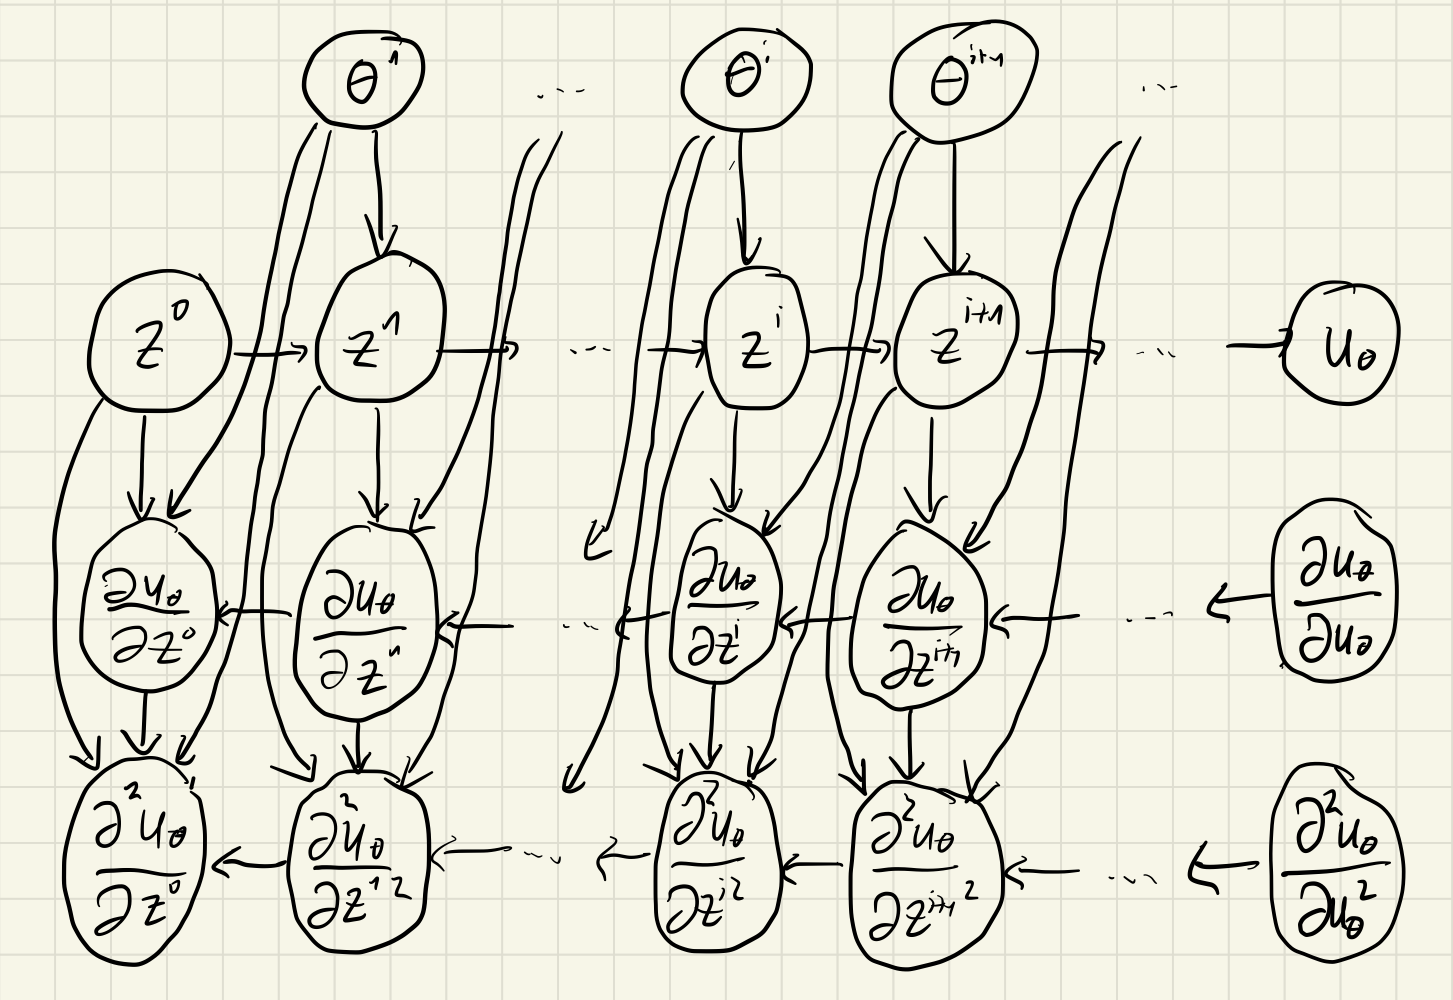
\includegraphics[width=0.6\linewidth]{figures/HBP_graph.png}
  \caption{Dependencies during gradient and Hessian backpropagation when computing the Hessian $\gradsquared{\vx}u_{\vtheta}$.}\label{fig:hbp-dependencies}
  \label{fig:hbp-dependencies}
\end{figure}

Following the procedure of \Cref{eq:hessian-backpropagation} yields the
per-layer parameter and feature Hessians $\gradsquared{\vz^{(i)}}u,
\gradsquared{\vtheta^{(i)}}u$. In \Cref{fig:hbp-dependencies} we depict the dependencies of
intermediate gradients and Hessians for computing $\gradsquared{\vx}u_{\vtheta}$:
\begin{itemize}
\item $\grad{\vz^{(i-1)}}u$ depends on $\grad{\vz^{(i)}}$ due to the recursion in \Cref{eq:gradient-backpropagation}, and on $\vz^{(i-1)}, \vtheta^{(i)}$ due to the Jacobian $\mJ_{\vz^{(i-1)}}\vz^{(i)}$ in the gradient backpropagation \Cref{eq:gradient-backpropagation}.

\item $\gradsquared{\vz^{(i-1)}}u$ depends on $\gradsquared{\vz^{(i)}}u$ and $\grad{\vz^{(i)}} u$ due to the recursion in \Cref{eq:hessian-backpropagation}, and on $\vz^{(i-1)}, \vtheta^{(i)}$ due to the Jacobian $\mJ_{\vz^{(i-1)}}\vz^{(i)}$ and Hessian $\gradsquared{\vz^{(i-1)}}[\vz^{(i)}]_k$ in the Hessian backpropagation \Cref{eq:gradient-backpropagation}.
\end{itemize}

\subsection{Laplacian}

The Laplacian $\Delta u_{\vtheta}$ follows by taking the trace of
$\gradsquared{\vx}u_{\vtheta}$ from above, and is hence recursively defined.

\begin{figure}[t]
  \centering
  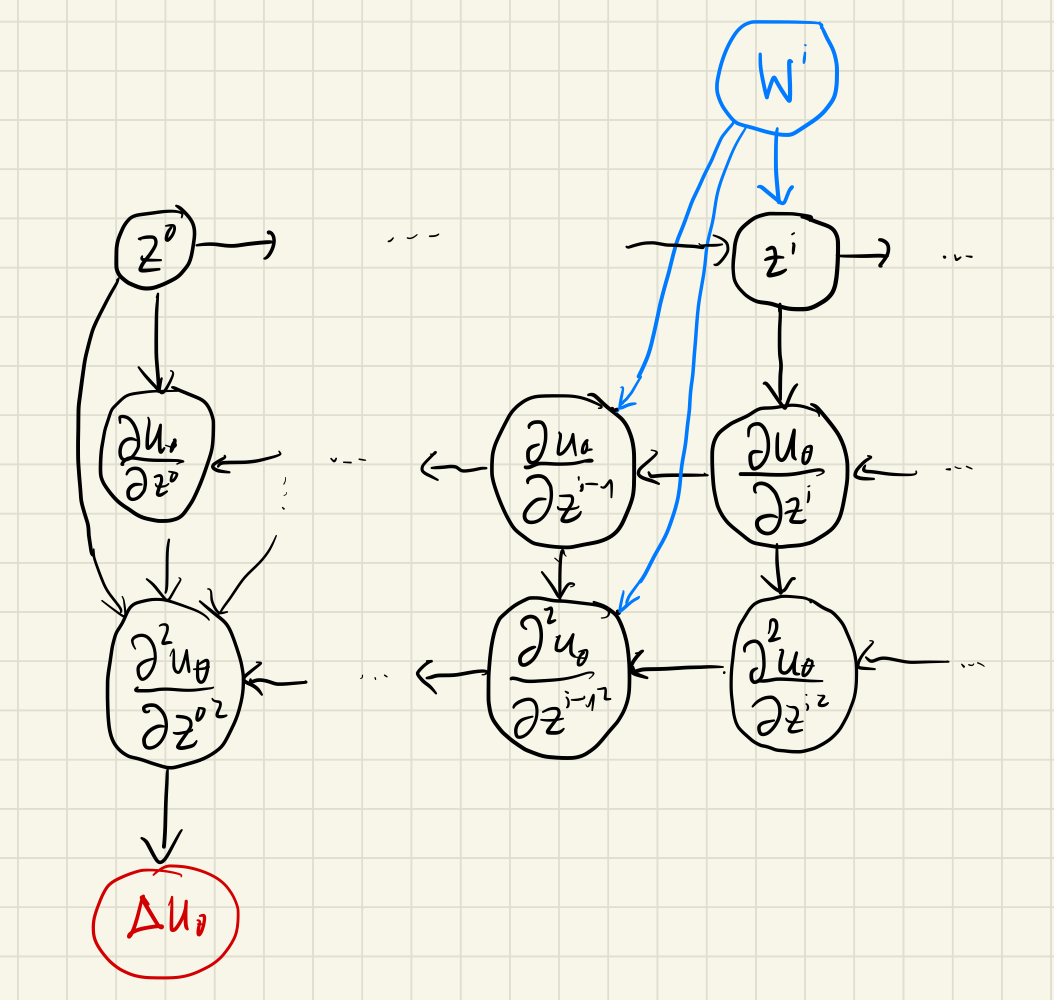
\includegraphics[width=0.6\linewidth]{figures/HBP_graph_weight.png}
  \caption{Direct children of the weight matrix of a single layer for the computation graph of the Laplacian.}\label{fig:laplacian-graph-weight}
\end{figure}

\paragraph{For a linear layer} To de-clutter the dependency graph of \Cref{fig:hbp-dependencies}, we will now consider the dependency of $\Delta u_{\vtheta}$ w.r.t.\,the weight of a single layer.
We assume this layer $i$ to be a linear layer with parameters $\mW^{(i)}$ such that $\vtheta^{(i)} = \flatten(\mW^{(i)})$,
\begin{align}
  \vz^{(i)} = \mW^{(i)} \vz^{(i-1)}\,.
\end{align}
For this layer, the second terms in \Cref{eq:hessian-backpropagation} disappears because the local Hessians are zero, that is $\gradsquared{\vz^{(i-1)}}[\vz^{(i)}]_k = \vzero$ and $\gradsquared{\mW^{(i)}}[\vz^{(i)}]_k = \vzero$.
Also, the Jacobians are $\jac_{\mW^{(i)}}\vz^{(i)} = {\vz^{(i-1)}}^{\top} \otimes \mI$ and $\jac_{\vz^{(i-1)}}\vz^{(i)} = \mW^{(i)}$ and hence only depends on one of the two layer inputs.
This simplifies the computation graph.
\Cref{fig:laplacian-graph-weight} shows the dependencies of $\mW^{(i)}$ on the
Laplacian, highlighting its three direct children,
\begin{align}
  \begin{split}
    \vz^{(i)}
    &=
      \mW^{(i)} \vz^{(i-1)}
    \\
    \grad{\vz^{(i-1)}}u
    &=
      {\mW^{(i)}}^{\top}
      \left(
      \grad{\vz^{(i)}}u
      \right)
    \\
    \gradsquared{\vz^{(i-1)}}u
    &=
      {\mW^{(i)}}^{\top}
      \left(
      \gradsquared{\vz^{(i)}}u
      \right)
      \mW^{(i)}
  \end{split}
\end{align}

\paragraph{Laplacian's derivative for a linear layer} We have now identified the direct children of $\mW^{(i)}$ in the Laplacian's compute graph.
This allows us to write down its derivative $\grad{\mW^{(i)}} \Delta u$, which---by the chain rule---is simply the accumulated backpropagated error from the direct children:
\begin{align}\label{eq:laplacian-gradient}
  \begin{split}
    \grad{\mW^{(i)}} \Delta u_{\vtheta}
    &=
      \sum_{\bullet \in \left\{ \vz^{(i)}, \grad{\vz^{(i-1)}}u, \gradsquared{\vz^{(i-1)}}u \right\}}
      \left(
      \jac_{\mW^{(i)}}\bullet
      \right)^{\top}
      \grad{\bullet}\Delta u
    \\
    &=
      \left(
      \jac_{\mW^{(i)}}\vz^{(i)}
      \right)^{\top}
      \grad{\vz^{(i)}}\Delta u
      +
      \left(
      \jac_{\mW^{(i)}}\grad{\vz^{(i)}}u
      \right)^{\top}
      \grad{\grad{\vz^{(i)}}u}\Delta u
      +
      \left(
      \jac_{\mW^{(i)}}\gradsquared{\vz^{(i)}}u
      \right)^{\top}
      \grad{\gradsquared{\vz^{(i)}}u}\Delta u\,.
  \end{split}
\end{align}

\paragraph{The Fisher} With the Laplacian's gradient \Cref{eq:laplacian-gradient}, we can write down the Fisher block for $\mW^{(i)}$
\begin{align}\label{eq:fisher}
  \begin{split}
    \mF^{(i)}
    &=
      \left(
      \grad{\mW^{(i)}} \Delta u_{\vtheta}
      \right)
      \left(
      \grad{\mW^{(i)}} \Delta u_{\vtheta}
      \right)^{\top}
    \\
    &=
      \sum_{\textcolor{blue}{\bullet} \in \left\{ \vz^{(i)}, \grad{\vz^{(i-1)}}u, \gradsquared{\vz^{(i-1)}}u \right\}}
      \sum_{\textcolor{red}{\bullet} \in \left\{ \vz^{(i)}, \grad{\vz^{(i-1)}}u, \gradsquared{\vz^{(i-1)}}u \right\}}
      \left(
      \left(
      \jac_{\mW^{(i)}}\textcolor{blue}{\bullet}
      \right)^{\top}
      \grad{\textcolor{blue}{\bullet}}\Delta u
      \right)
      \left(
      \left(
      \jac_{\mW^{(i)}}\textcolor{red}{\bullet}
      \right)^{\top}
      \grad{\textcolor{red}{\bullet}}\Delta u
      \right)^{\top}
    \\
    &=
      \sum_{\textcolor{blue}{\bullet} \in \left\{ \vz^{(i)}, \grad{\vz^{(i-1)}}u, \gradsquared{\vz^{(i-1)}}u \right\}}
      \sum_{\textcolor{red}{\bullet} \in \left\{ \vz^{(i)}, \grad{\vz^{(i-1)}}u, \gradsquared{\vz^{(i-1)}}u \right\}}
      \underbrace{
      \left(
      \jac_{\mW^{(i)}}\textcolor{blue}{\bullet}
      \right)^{\top}
      \left[
      \left(
      \grad{\textcolor{blue}{\bullet}}\Delta u
      \right)
      \left(
      \grad{\textcolor{red}{\bullet}}\Delta u
      \right)^{\top}
      \right]
      \left(
      \jac_{\mW^{(i)}}\textcolor{red}{\bullet}
      \right)}_{
      := \mF^{(i)}_{\textcolor{blue}{\bullet}, \textcolor{red}{\bullet}}
      }\,.
  \end{split}
\end{align}
The Fisher consists of nine different terms.
Eventually, we would like to approximate it with a single Kronecker product, like KFAC~\citep{martens2015optimizing}.
Note that one of the nine terms is the term from the original KFAC paper, namely
when $\textcolor{blue}{\bullet} = \textcolor{red}{\bullet} = \vz^{(i)}$
(remember that $\jac_{\mW^{(i)}} \vz^{(i)} = \vz^{(i-1)} \otimes \mI$):
\begin{align}\label{eq:original-kfac}
  \begin{split}
    \mF^{(i)}_{\textcolor{blue}{\vz^{(i)}}, \textcolor{red}{\vz^{(i)}}}
    &=
      \left(
      \textcolor{blue}{\vz^{(i-1)} \otimes \mI}
      \right)
      \left[
      \left(
      \textcolor{blue}{\grad{\vz^{(i-1)}}\Delta u}
      \right)
      \left(
      \textcolor{red}{\grad{\vz^{(i-1)}}\Delta u}
      \right)^{\top}
      \right]
      \left(
      \textcolor{red}{{\vz^{(i-1)}}^{\top} \otimes \mI}
      \right)
    \\
    &=
      \textcolor{blue}{\vz^{(i-1)}}
      \textcolor{red}{{\vz^{(i-1)}}^{\top}}
      \otimes
      \left(
      \textcolor{blue}{\grad{\vz^{(i-1)}}\Delta u}
      \right)
      \left(
      \textcolor{red}{\grad{\vz^{(i-1)}}\Delta u}
      \right)^{\top}
    \\
    &:= \mA_{\text{KFAC}}^{(i)} \otimes \mB_{\text{KFAC}}^{(i)}\,.
  \end{split}
\end{align}
\Cref{eq:original-kfac} illustrates that the Kronecker structure emerges from
the Jacobians. So we need to investigate these objects closer for the remaining
terms of \Cref{eq:fisher}.

\paragraph{Jacobians from the gradient and Hessian backward pass} We already know the Jacobian from the linear layer's forward pass,
\begin{subequations}\label{eq:fisher-jacobians}
  \begin{align}
    \jac_{\mW}\left( \mW \vx \right) = \vx^{\top} \otimes \mI\,.
  \end{align}
  The Jacobian from the gradient backpropagation is
  \begin{align}
    \jac_{\mW}\left( \mW^{\top} \vx \right) = \mI \otimes \vx^{\top}\,,
  \end{align}
  and the Jacobian from the Hessian backpropagation is
  \begin{align}
    \jac_{\mW}\left( \mW^{\top} \mX \mW \right) = \mI \otimes \mW^{\top}\mX + \mI \otimes \mW^{\top}\mX^{\top}\,.
  \end{align}
\end{subequations}
\toodoo{F.D.\,derived the Jacobians from \Cref{eq:fisher-jacobians} by hand.
  Might be worth to double-check for correctness.}
The Jacobians from \Cref{eq:fisher-jacobians} allow to express the Fisher in
terms of Kronecker-structured expressions consisting of 16 terms in total.

\toodoo{F.D.\,Write down the full expression for the Fisher.
  Propose ways to Kronecker-approximate each of the 16 terms, such that we end up with a single Kronecker product in the end.}

%%% Local Variables:
%%% mode: latex
%%% TeX-master: "../main"
%%% End:


\bibliography{references}
\bibliographystyle{apalike}
\end{document}

%%% Local Variables:
%%% mode: latex
%%% TeX-master: t
%%% End:
